\subsection{Objects features}
% \begin{figure}
%     \centering
%     \subfloat[Area]{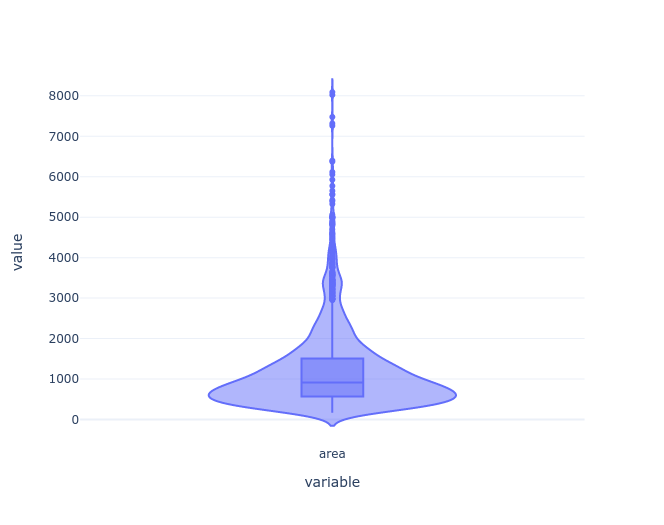
\includegraphics[width=0.5\textwidth]{figures/120_dataset/geometric_features area.png}
%     \label{fig:dataset:geom:area}
%     }
%     \subfloat[Feret diameter]{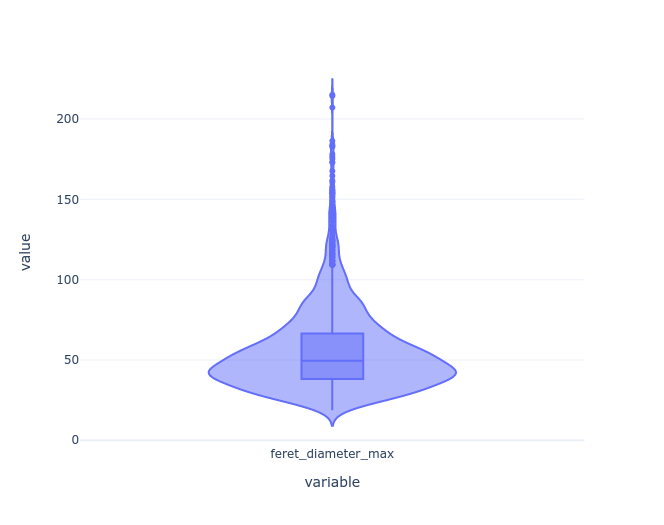
\includegraphics[width=0.5\textwidth]{figures/120_dataset/geometric_features feret.png}
%     \label{fig:dataset:geom:feret}
%     }
%     \caption{\textbf{Geometrical features.} Distributions of the area (left) and maximum Feret diameter (right) across all annotated cells.}
%     \label{fig:dataset:geom}
% \end{figure}
\begin{figure}
    \centering
    \subfloat[Area]{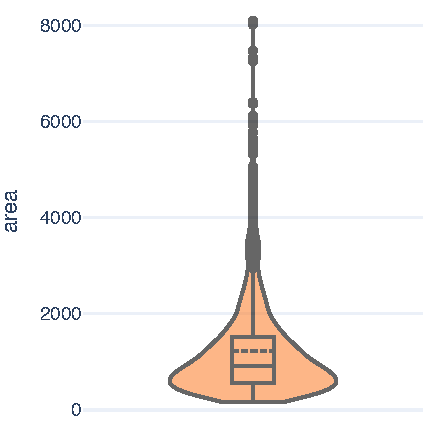
\includegraphics[width=0.5\textwidth]{figures/120_dataset/features/area.pdf}
    \label{fig:dataset:geom:area}
    }
    \subfloat[Feret diameter]{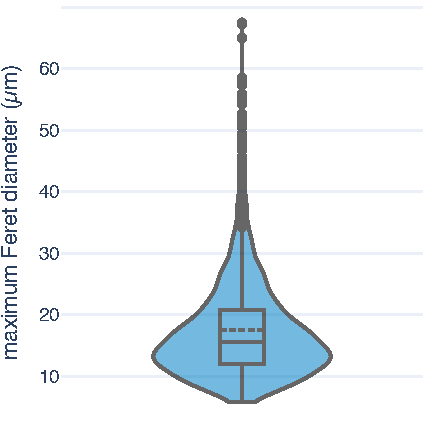
\includegraphics[width=0.5\textwidth]{figures/120_dataset/features/feret_diameter.pdf}\label{fig:dataset:geom:feret}
    }
    \caption{\textbf{Geometrical features.} Distributions of the area (left) and maximum Feret diameter (right) across all annotated cells.}
    \label{fig:dataset:geom}
\end{figure}
After the initial exploration of the data characteristics at the pixel level, additional investigations can be devoted to discovering meaningful insights about images' macroscopic content.
The Fluorescent Neuronal Cells pictures present a rich collection of 2137 neuronal cell instances of various shapes and sizes (see \textit{area}, and \textit{Feret diameter} columns in \cref{tab:data_features} for a numeric summary) that are unevenly distributed across the images.

\Cref{fig:dataset:geom} shows the distributions of the most interesting geometrical features of the annotated objects.
Regarding the area distribution (\cref{fig:dataset:geom:area}), the bulk of the distribution presents cells with a surface within 358 and 1504 pixels.
\Cref{fig:dataset:geom:feret} reports the maximum Feret diameter \cite{merkus2009particle} instead. This measure is computed as the longest distance (in pixels) between points of a convex cell countour\footnote{obtained using skimage package version `0.18.1'}.
The distribution extends from a minimum of 18 to a maximum of 215 pixels, with the central 50\% concentrated in the range [38, 66].
In both cases, the distribution is left-skewed, with a slight prevalence of values lower than the median.
In fact, 90\% of objects are small and medium cells with prevalently regular circular shapes, having an area within [162, 2409] pixels and a Feret diameter between 18 and 88.
The remaining 10\% of the distribution stretches up to a maximum of 8092 and 215, respectively.
This effect is due to the contribution of more oversized or prolonged objects that cause a long, heavy tail.

Finally, \ref{fig:dataset:counts_distrib} illustrates the distribution of the number of cells across the dataset (see \textit{\# cells} columns in \cref{tab:data_features} for a numeric summary).
In this case, the distribution presents multiple modes that can be summed up by the five major peaks, namely 6, 35, 38, 53 and 68
(\cref{fig:dataset:counts_hist}).
The empty spaces are a consequence of the fact that not all of the possible values were actually observed in the data.
Interestingly, a lower peak is observed at 0 because of the 56 images where no cells were annotated.

By looking at the estimated density in the violin plot (\cref{fig:dataset:counts_violin}), it appears that the distribution can be interpreted as a mixture of two components.
%In particular, one can distinguish two peaks by looking at the estimated density in \cref{fig:dataset:counts_violin}.
The first is centered around 6 and is made of the images with lower counts, i.e. the ones depicting brain areas where the fluorophore did not yield abundant emissions.
The second, instead, is a combination of the four higher peaks that represent active brain areas.
% \begin{figure}
%     \centering
%     \subfloat[Histogram]{
%     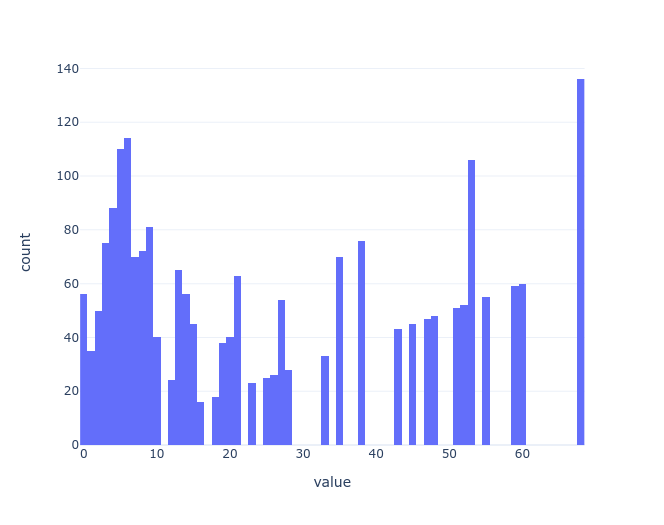
\includegraphics[width=0.5\textwidth]{figures/120_dataset/counts_histogram.png}
%     \label{fig:dataset:counts_hist}
%     }
%     \subfloat[Violin plot]{
%     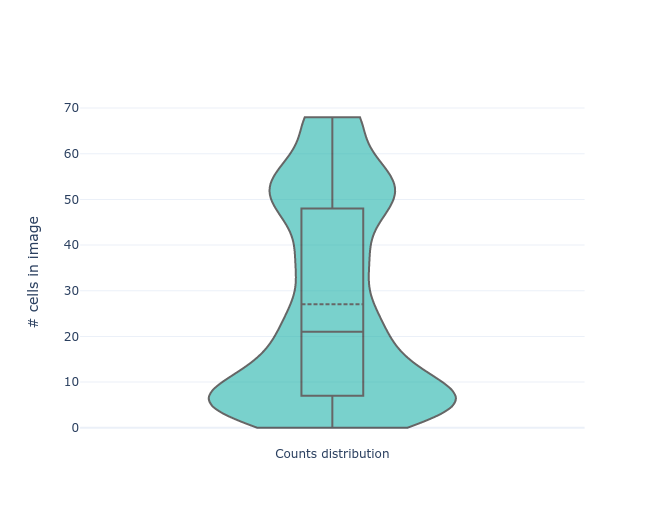
\includegraphics[width=0.5\textwidth]{figures/120_dataset/counts_violin.png}
%     \label{fig:dataset:counts_violin}
%     }
%     \caption{\textbf{Counts distribution.} Distributions of the number of annotated cells across all images in the dataset.}
%     \label{fig:dataset:counts_distrib}
% \end{figure}


\begin{figure}
    \centering
    \subfloat[Histogram]{
    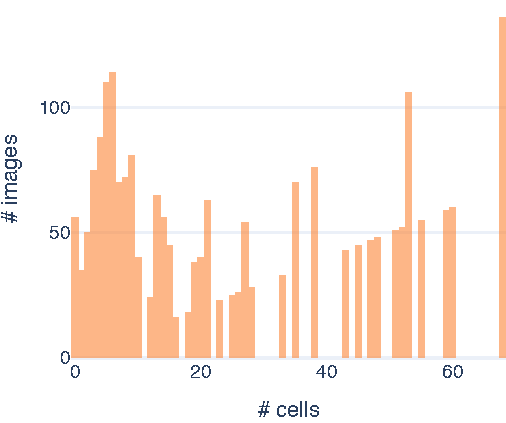
\includegraphics[width=0.6\textwidth]{figures/120_dataset/features/count_histogram.pdf}
    \label{fig:dataset:counts_hist}
    }
    \subfloat[Violin plot]{
    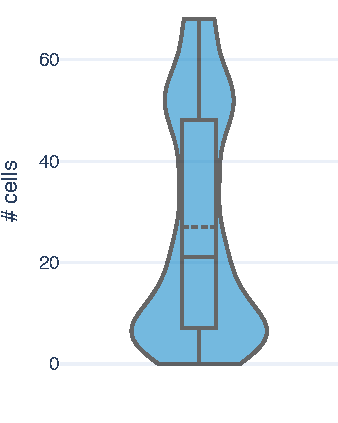
\includegraphics[width=0.4\textwidth]{figures/120_dataset/features/count_violin.pdf}
    \label{fig:dataset:counts_violin}
    }
    \caption{\textbf{Counts distribution.} Distributions of the number of annotated cells across all images in the dataset.}
    \label{fig:dataset:counts_distrib}
\end{figure}